\newgeometry{margin=1cm}%

%%%%%%%%%%%%%%%%%%%% Title page %%%%%%%%%%%%%%%%%%%%
\vspace*{0.05\textheight}
{\centering
{\fontsize{46}{60}\fontseries{b}\selectfont%
Homotopy Type Theory}\par
\vspace*{20pt}
{\fontsize{23}{40}\fontseries{b}\fontshape{sc}\selectfont%
Univalent Foundations of Mathematics}\par
\vfill
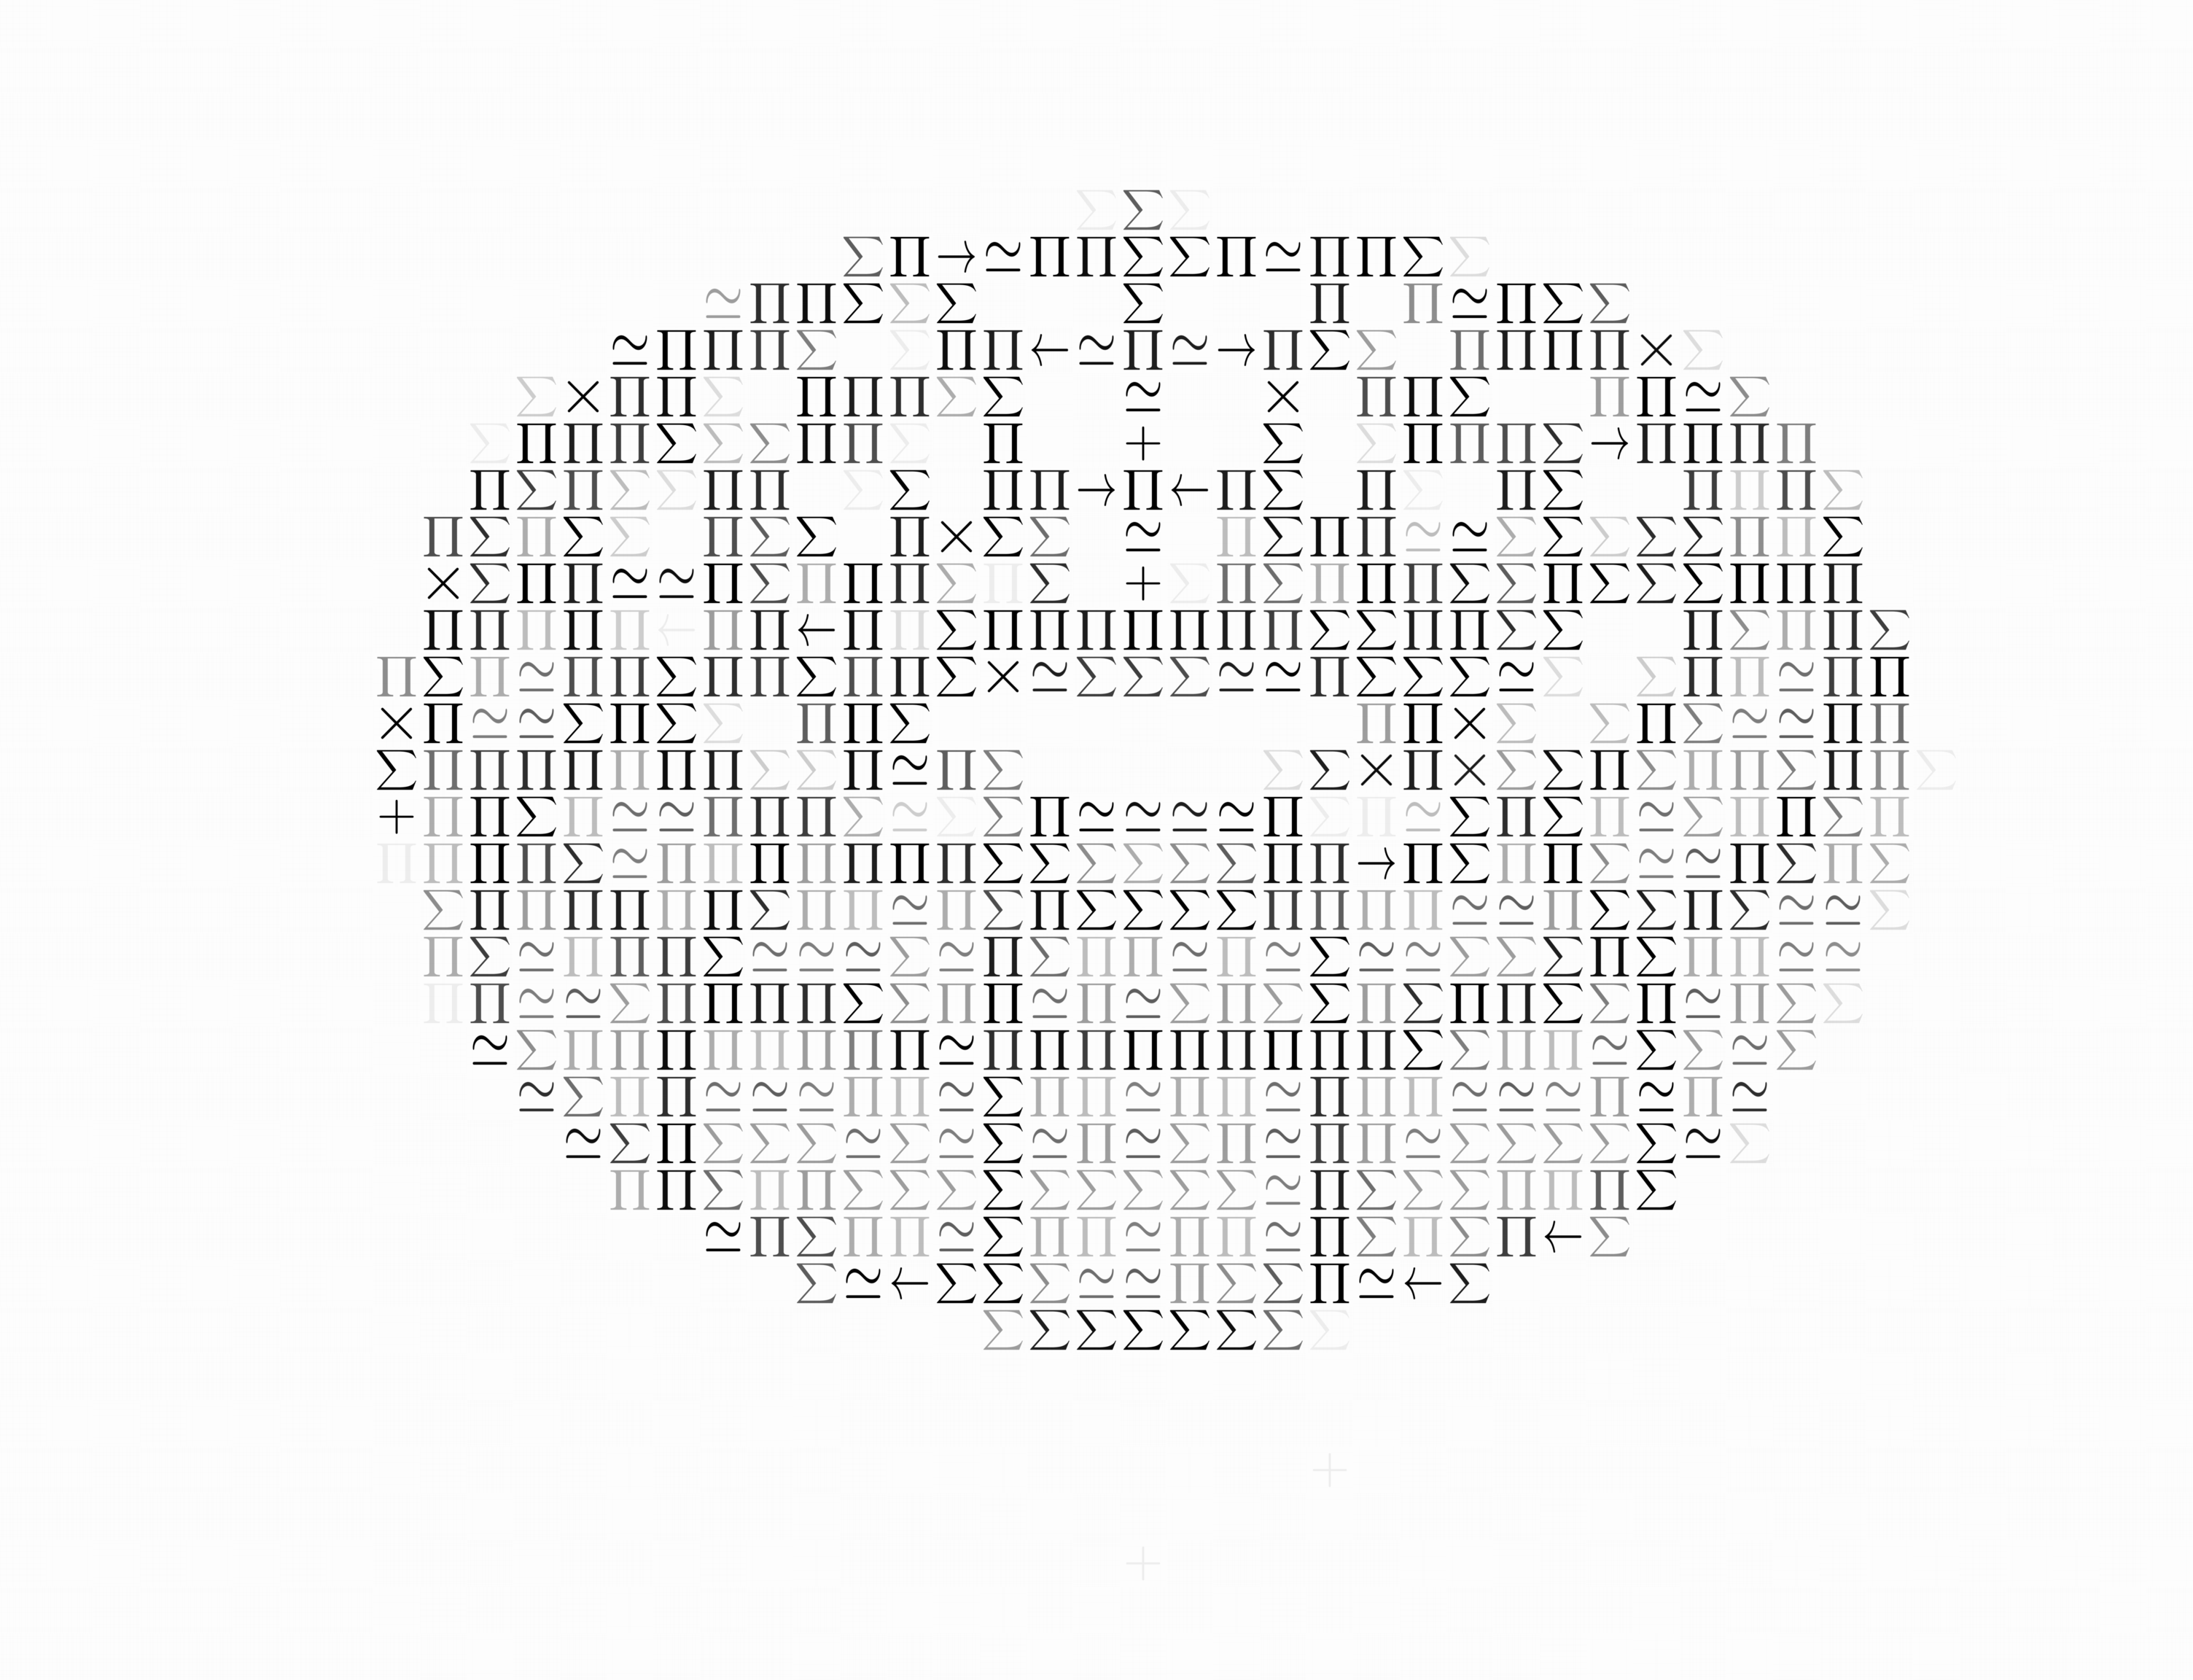
\includegraphics[width=\textwidth]{cover.png}
\vfill
{\fontsize{19}{25}\fontshape{n}\selectfont%
The Univalent Foundations Program\par
\vspace*{8pt}
Institute for Advanced Study\par
}}
\vspace{0.05\textheight}
\hbox{}

\clearpage
%%% Restore page style
\restoregeometry

%%%%%%%%%%%%%%%%%%%% Copyright page %%%%%%%%%%%%%%%%%%%%
\hbox{}
\vfill

{\footnotesize
\noindent
\emph{``Homotopy Type Theory: Univalent Foundations of Mathematics''}\\
\copyright\ 2013 The Univalent Foundations Program

\bigskip

\noindent
\emph{``Flames''} cover page photo\\
\copyright\ 2013 Jordan Smith of \href{http://rippah2.deviantart.com/}{rippah2.deviantart.com}

\bigskip

\noindent
This book is freely available at
{\tt homotopytypetheory.org}.
%

\bigskip

\noindent
This work is licensed under the
\textbf{\emph{Creative Commons Attribution-ShareAlike 3.0 Unported License.}}
%
To view a copy of this license, visit
\href{http://creativecommons.org/licenses/by-sa/3.0/}{http://creativecommons.org/licenses/by-sa/3.0/}.
The following is a human-readable summary of the Legal Code (the full license).

\bigskip

\noindent
\emph{You are free:}
%
\begin{description}
\item[to Share] --- to copy, distribute and transmit the work,
\item[to Remix] --- to adapt the work to make commercial use of the work.
\end{description}
%
\emph{Under the following conditions:}
%
\begin{description}

\item[Attribution] --- You must attribute the work in the manner specified by the author
  or licensor (but not in any way that suggests that they endorse you or your use of the
  work).

\item[Share Alike] --- If you alter, transform, or build upon this work, you may
  distribute the resulting work only under the same or similar license to this one.
\end{description}
%
\emph{With the understanding that:}
\begin{description}

\item[Waiver] --- Any of the above conditions can be waived if you get permission from the
  copyright holder.

\item[Public Domain] --- Where the work or any of its elements is in the public domain
  under applicable law, that status is in no way affected by the license.

\item[Other Rights] --- In no way are any of the following rights affected by the license:
  \begin{itemize}
  \item Your fair dealing or fair use rights, or other applicable copyright exceptions and
    limitations;
  \item The author's moral rights;
  \item Rights other persons may have either in the work itself or in how the work is
    used, such as publicity or privacy rights.
  \end{itemize}
\end{description}
}
\cleartooddpage

%%% Local Variables: 
%%% mode: latex
%%% TeX-master: "main"
%%% End: 
